\chapter{Cahier des charges}
\section*{Chronogramme}
\begin{center}
\end{center}
\section{Remise en contexte}
\paragraph{Les vulnérabilités de type Use-After-Free}
\subparagraph{}
La plupart des vulnérabilités enseignées et étudiées dans le cadre scolaire
se rapportent à des fonctionnement souvent statique, ou du moins dont le comportement
est uniquement lié au programme ciblé en lui-même (à son architecture de compilation et/à
son code source). On prendra comme exemple les dépassements de tampons, les problèmes de
formatage des chaines de caractères, etc.\subparagraph{}
Dans l'environnement industriel, et sur les solutions importantes utilisées dans le monde
de l'entreprise, ces vulnérabilités sont de plus en plus rare. Premièrement parce que le temps
faisant son œuvre, la grande majorité ont été reportées sur les solutions les plus anciennes,
mais également parce que de nombreux outils pouvant les détecter rapidement (parfois dès la compilation)
ont été conçus.\subparagraph{}
Les attaquants explorent donc de nouvelles voies, notamment sur des problématiques plus dynamiques, et/ou
lié également à l'environnement de production du programme, comme le système d'exploitation ou la bibliothèque utilisée.
En effet, de nombreuses opérations du programme dépendent intrinsèquement du système d'exploitation sous-jacent et
même si le comportement final reste souvent le même sur les différentes plateformes, les effets collatéraux
sur le contexte et le mécanisme d'exécution est souvent différent.\subparagraph{}

\subparagraph{L'évolution des vulnérabilités de type use-after-free}
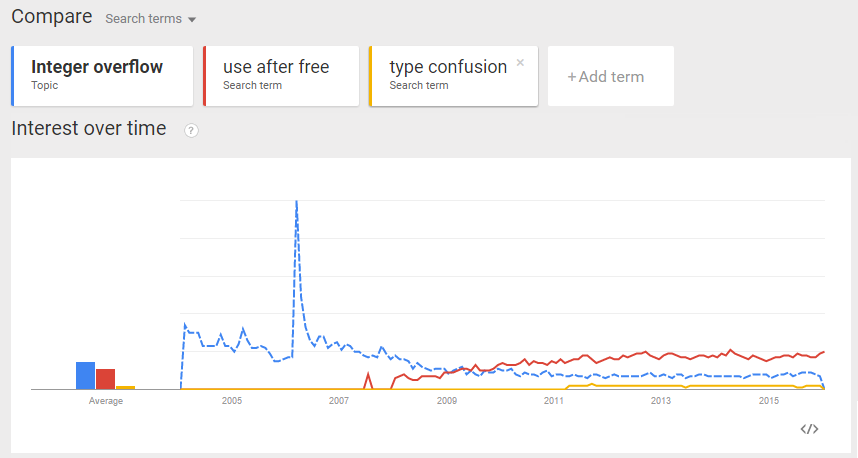
\includegraphics[scale=0.5]{histogramme-uaf.png}\newline
Beaucoup de problème de corruption mémoire sont directement dû à la mauvaise utilisation
du langage utilisé pour le développement. En effet, les langages de programmation tels que C
ou C++ demandent une gestion de la mémoire manuelle (le C++ permet néanmoins une gestion plus ou moins automatisée
avec les nouveaux standards).
\subparagraph{}
Il est donc fréquent de rencontrer des erreurs sur ce point là. Cela arrive
notamment lorsque par un problème de maintenabilité ou de mauvaise conception, la partie du programme devant
libérer une zone mémoire est méconnue/non documentée.\subparagraph{}
Ce n'est cependant pas toujours le cas et les allocateurs de mémoires / ramasse-miettes sont parfois en cause.

\subparagraph{Exemple}
Un exemple très simple et souvent rencontré dans la littérature est le suivant:
\begin {lstlisting}[frame=single]
int main(void)
{
    int *a = malloc(sizeof(int));
    *a = 5;
    free(a);
    int *b = malloc(sizeof(int));
    printf("\%d", *b); // affiche 5
    *b = 7;
    printf("\%d", *b); // affiche 7
    *a = 10;
    printf("\%d", *b); // affiche 10
}
\end{lstlisting}
\subparagraph{}
Sur une distribution Linux classique comme Ubuntu, quelque soit la taille de mots
de l'architecture (32 ou 64 bits), les adresses a et b sont exactement les mêmes.
Cela est directement dû à l'algorithme d'allocation mémoire de la bibliothèque standard
C.\subparagraph{}
En effet lors du premier appel à la fonction \textbf{malloc()}, une première zone est allouée.
Lors de sa libération, la zone libérée est mise en cache, et lors du second appel à \textbf{malloc()},
l'algorithme va retourner la même zone mémoire. Ce comportement ne sera pas détaillée dans cette section, car
il demanderait à lui seul plusieurs pages.\subparagraph{}
Cela va de soi que cet exemple est simpliste, et que les vulnérabilités rencontrées en production sont
rarement aussi visible. Il permet toutefois de bien visualiser l'origine du problème.


\paragraph{Outils existants en dynamique et en statique}
Des outils simplistes ne suffisent pas à détecter la présence d'use-after-free.\newline
Par exemple, si une solution détecte uniquement l'accès à une zone mémoire non allouée, l'exemple
donnée précédemment ne sera pas considéré comme vulnérable, car la zone mémoire est là même pour deux
allocations différentes. Plusieurs possibilités s'ouvrent alors : l'analyse statique, l'analyse dynamique,
et un mélange des deux.

\paragraph{Analyse dynamique}
De nombreuses personnes / équipes se sont penchées sur la détection de ces comportements, dynamiquement et
statiquement. Nous parlerons tout d'abord des solutions dynamiques existantes, puis nous aborderons \textbf{les approches
statiques, qui sont directement liées au sujet de ce stage.}

\subparagraph{Kasan: Kernel Address Sanitizer}
Kasan est un projet open-source, développée majoritairement
par les acteurs du noyaux Linux ainsi que par Google. Son but est d'ajouter une couche de protection
mémoire au noyau Linux afin de détecter certains corruptions mémoires dans les opérations du noyau, comme
des use-after-free ou des accès hors limites.
https://github.com/google/kasan

\subparagraph{AddressSanitizer}
AddressSanitizer est également un projet open-source, et effectue
un travail similaire à Kernel Adress Sanitizer. Intégré dans la base de code de
LLVM, il permet, lorsque le programme testé est compilé avec les bonnes options du compilateur \textbf{Clang},
de détecter des problèmes de mémoires.

\subparagraph{Undangle}
Undangle est également un exemple connu, spécialement dédié à la découverte de vulnérabilité
de type use-after-free et double-free, à partir d'une trace d'exécution. Il a été développé par plusieurs
personnes travaillant à l'IMDEA Software Institute.

\paragraph{Analyse statique}

De nombreux outils dynamique détectant les problèmes liés à la mémoire existent et remplissent parfaitement leur rôle.
L'analyse dynamique a néanmoins plusieurs défauts.\newline

\subparagraph{Les avantages d'une analyse statique}

Lors de la phase de test d'une application, ainsi que lors de la recherche de vulnérabilités dans celle-ci, une bonne méthodologie
est d'essayer de parcourir tous les chemins possibles lors de l'exécution. Cela nécessite donc plusieurs répétitions, ainsi qu'une connaissance
pointue du programme en lui même.\newline
Cependant, il est théoriquement impossible de parcourir tous les options possibles d'un programme, notamment si
celui-ci dépend d'entrées utilisateurs ou de paramètre du système sur lequel il opère. Cela est d'autant plus vrai lorsque le binaire atteint une taille
considérable. De plus, les bonnes suite de tests se font extrêmement rare au niveau professionnel.

\subparagraph{Les inconvénients d'une analyse statique}

Malgré le fait qu'une analyse statique autorise théoriquement le parcours de tous les chemins d'exécution existant, plusieurs obstacles
limite parfois son utilité.\newline

Les corruptions mémoires sont par nature dynamiques. Lorsqu'une allocation s'effectue, son emplacement n'est pas prédéterminé
et plusieurs facteurs extérieurs peuvent venir gêner l'opération (absence d'espace mémoire). De plus, une allocation
est essentiellement liée à sa taille, et le dépassement de tampons et autres vulnérabilités se basent souvent sur cette information.
Lors d'une analyse statique, cette taille n'est pas forcement connue, à part dans quelques cas précis.
\subparagraph{}

En dehors des contraintes sur la précision de l'analyse, une des limitations de l'analyse statique repose sur le système et l'algorithme
dévoué à l'analyse. Prendre plusieurs chemins et conserver les états, répertorier l'ensemble de ces informations en mémoire, l'analyse
statique de boucles, et autres, peuvent prendre une taille considérable en mémoire, et souvent, un compromis doit se faire entre la vitesse
d'analyse et la mémoire allouée au programme. Sur certains binaires, l'analyse peut durer plusieurs jours. Durant les tests réalisés pendant le
stage, les douze giga de mémoire étaient parfois atteints.

\subparagraph{}
Lorsqu'un binaire ou sa trace d'execution possible est analysé, surtout lorsque le traitement est général et sans destination précise (c'est à dire
qu'aucune instruction particulière dans le binaire n'est visée). On se retrouve alors face au problème d'"explosion de chemins (path explosion).

\subparagraph{}
Ces problématiques d'espace, d'analyse de boucles et d'optimisation de temps ont occupé une grande partie de ce stage et seront développées plus
en détails lors des prochaines sections de ce rapport.

\subparagraph{Les outils statiques existants} sont plutôt rare comparés à la masse d'analyseur dynamiques. Néanmoins certains sortent du lot.

\subparagraph{GUEB}
GUEB a été développé principalement par Feist Josselin durant sa thèse. Il se base sur une représentation intermédiaire
REIL fournie par l'outil BinNavi. En se basant sur cette représentation, l'outil parcours le binaire pour retrouver des vulnérabilités
de type use-after-free possibles.

\section{Présentation globale du projet}
\paragraph{Un analyseur statique}

Le projet de ce stage fut de développer en Python2.7 un analyseur statique de fichier
binaire exécutable afin de détecter des vulnérabilités de type use-after-free sans aide
provenant de rapports fournis par des outils externes.

\paragraph{Ambition}

Comme évoquée dans la section précédente de ce rapport, une analyse statique complète est souvent
longue et très demandante en ressources. Les connaissances en début de stage sur le sujet étant limitées,
une phase d'apprentissage étant indispensable (retirant donc du temps de développement), l'ambition du stage
a donc été revue en conséquence.
\subparagraph
Plusieurs objectifs étaient fixés concernant la globalité du projet:
\begin{itemize}
        \item Une montée en compétence sur le sujet
        \item Un outil fonctionnel même si long à l'analyse
        \item Une base maintenable, documentée et reprenable dans des travaux futurs
\end{itemize}

Il était attendu qu'à la fin du stage, ces points la soient acquis. Le côte "fonctionnel"
de l'outil était cependant laissé volontairement vague. Les fonctionnalités mises en place
devaient exister, en étant aussi performante que possible, mais le développement devait se faire
pas à pas, et la qualité d'une fonctionnalité primait sur l'accumulation de plusieurs autres.

\section{Résultat à obtenir}
\paragraph{Objectifs d'utilisation de l'outil}

\subparagraph{Différence par rapport à l'existant}

Quasiment toutes les solutions existantes se basent sur un rapport ou une représentation agrémentée d'informations fournis
par un outil extérieur, effectuant déjà une première analyse, tel qu'IDA ou BinNavi. Un des premiers objectifs étaient donc de
se baser uniquement sur une aide externe pouvant fournir le \textbf{désassemblage} du binaire ainsi qu'une \textbf{representation intermédiaire}
pour plus de généricité au regard de l'architecture ciblée par le binaire.

\subparagraph{Format(s) visé(s)}

Les deux formats de fichier les plus courants en entreprises, PE et ELF étaient la priorité principale. Le format mach-o pour
Mac OS X n'était pas envisagé, ne serait ce qu'a cause du peu de désassembleurs supportant ce format. La différence de traitement
entre les formats d'exécutables réside quasi uniquement dans la récupération des symboles et de la table d'import. En effet, ceux-ci
sont stockés différemment selon le format, et sont indispensables pour garder la trace des fonctions allouant ou libérant de la mémoire.

\subparagraph{Architecture(s) visé(s)}
Les architectures que l'ont peu trouver sur le marché sont nombreuses et correspondent souvent à un usage bien spécifique.
Les ordinateurs de bureau et ordinateurs portables sont majoritairement équipés d'architecture x86-(64), et on retrouve de plus en plus
cet architecture sur certains serveurs, grâce à leur performance et leur prix. Les téléphones portables préfèrent souvent quand à eux
des architectures comme ARM qui consomment moins d'énergie. Ces deux architectures été initialement choisis pour l'analyseur, mais seul
le fonctionnement sur architecture x86 a été testé. Néanmoins, le support pour ARM est assuré par une abstraction par rapport aux systèmes
sous-jacents.
\subparagraph{}
La différence entre deux architectures se fait surtout sur les conventions d'appels qui peuvent les accompagner, comme le registre accueillant
la valeur de retour d'une fonction, ou les registres contrôlant la pile. Le reste des registres sont abstraits et sont de toute manière
juste traités comme des identifiants lors de l'analyse.


\chapter{Compte-rendu d'activité}
\section{Compréhension des allocateurs mémoire}
Lors de son execution, un programme est chargé en mémoire et le système d'exploitation
met à sa disposition un espace mémoire (que l'on parle de mémoire virtuelle ou physique)
d'une certaine taille. Cet espace est découpé en plusieurs parties : les segments du programme
(segment de code, segment de données, segment de pile, segment de tas), son tas et sa pile. Si les segment de code et de
données et garde généralement la même taille pour le temps de l'execution, les segments de pile et de tas sont par définition
dynamique et peuvent s'élargir ou rétrécir. Même s'il est possible d'augmenter la taille de la pile de manière dynamique (grâce
à la fonction \textbf{alloca()} sur des systèmes UNIX par exemple), son utilisation n'est pas encouragé pour stocker des données
dynamiques. Le tas, quand à lui, est un espace mémoire spécialement réservé pour cet emploi.
\begin{center}
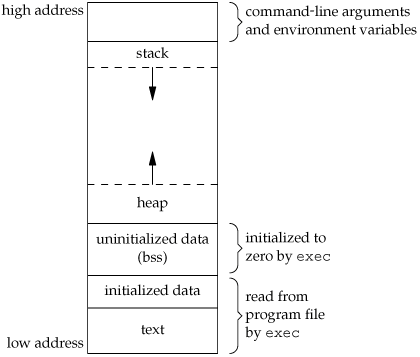
\includegraphics[scale=0.4]{memory-layout.png}\newline
\end{center}


\paragraph{Allocation et Libération: base des algorithmes}
\subparagraph{Allocation sur le tas}
Une des fonctions les plus connues des programmeurs et ingénieurs sous environnement UNIX est \textbf{malloc()} (respectivement \textbf{HeapAlloc()} sur
environnement Windows). En effet, en espace utilisateur, cette fonction est la base de l'allocation mémoire dynamique. Comme beaucoup de fonctions
manipulant le système d'exploitation et l'architecture sous-jacente, \textbf{malloc()} conserve son état tout au long de l'execution et répertorie les
changements dans des données réservés à son utilisation (première zone libre, pointeurs sur une structure de base, etc...).
\subparagraph{}
Il existe de nombreuses alternatives au classique \textbf{malloc()}, provenant de bibliothèque externe et permettant de s'adapter aux besoins, voir d'améliorer les
performance globales (\textbf{gmalloc()}, \textbf{TCmalloc()}. Néanmoins, la base de l'algorithme reste le même quelque soit la bibliothèque utilisée.

\subparagraph{Découpage en bloc du tas}
Pour gérer les allocations de différentes tailles, l'allocateur mémoire découpe au fur et à mesure des demandes
le segment qui lui est réservé. Ce découpage donne formation à des blocs mémoires qui sont marqués comme libre ou alloué, en gardant leur taille respective
en information.
\subparagraph{}
Pour plus de rapidité lors de l'allocation et la libération, des liens sont conservés entre les différents blocs libres (suivant et précédent). Ainsi lors d'une allocation,
un parcours simple à partir du premier bloc libre permet de trouver un espace convenant à la demande. D'autres informations peuvent être stockées selon l'implémentation.
Un des exemples le plus courant est le suivant\footnote{http://gee.cs.oswego.edu/dl/html/malloc.html}:
\begin{center}
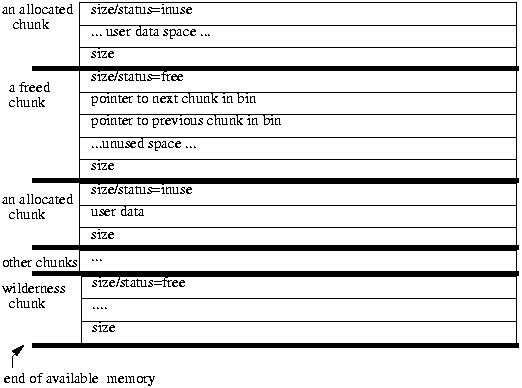
\includegraphics[scale=0.5]{malloc.png}\newline
\end{center}

On remarque l'optimisation de l'espace pour les blocs libres. Au lieu d'utiliser de l'espace dans le cas général, qui ne servirait pas dans le cas des blocs alloués,
on préfère placer les pointeurs vers les autres blocs libres à l'intérieur de l'espace libre. Cela amenera d'ailleurs une discussion sur la granularité des allocations dans
les prochains paragraphes.
\subparagraph{}
La taille est également stockée au début et à la fin d'un bloc. Cela permet une coalescion plus simple des blocs libres. En effet quand deux blocs contigus en
mémoire sont libres, il est possible des les réunir en un seul plus gros blocs.

\subparagraph{Optimisation : cache}
Cette algorithme a cependant des limites. Si la fréquence d'allocation est rapide, et si les tailles allouées/libérés sont très variées, on retrouve un phénomene de
fragmentation important, et les blocs libres restant peuvent être trop petit pour une prochaine allocation, même s'ils auraient pu collectivement suffire.
\subparagraph{}
Pour assurer une fragmentation moins importante, la plupart ont mis au point un système de cache (look-aside lists puis Low Fragmentation Heap sur Windows, différents sur Linux).
Le principe est simple : l'allocateur garde une liste des blocs libres d'une certaines tailles. Selon l'algorithme utilisé, les tailles pré-alloués peuvent différées.
On peut découper ces stratégies de caches en deux: la refonte différé et la pré-allocation.

\subparagraph{Refonte différé}
Au lieu de faire une refonte des blocs contigus lors de la libération, les blocs sont conservés libres et indépendent, et rajouté à la liste des blocs libres de
la taille correspondante. Cela dans l'espoir que les prochaines allocations utiliseront une taille proche.

\subparagraph{Pré-Allocation}
Plutôt que d'attendre une libération, une partie de la mémoire initiale est pré-découpée pour remplir les caches. L'autre partie est conservé pour les allocations
ne rentrant pas dans les catégories mises en cache.

\subparagraph{}
Ce principe de cache est notamment très utile dans les environnements où la même taille est alloué un très grand nombre de fois. On peut imaginer par exemple un
algorithme allouant une structure pour chacun des utilisateurs s'enregistrant sur une application, ou simplement un service allouant la même taille un très grand nombre
de fois pour y stocker des messages. En terme de statistique, un programme a souvent un spectre de taille d'allocation réduit, ce qui a conduit à la présence systèmatique de
cache dans les algorithmes d'allocation mémoire.


\subparagraph{Granularité des allocations}
Comme évoqué précedemment, la granularité des blocs alloués peut varier selon les méthodes et les allocateurs utilisés. La "granularité" d'une allocation
correspond à une taille fixe dont la taille d'une allocation sera un multiple. En effet, même si l'utilisateur demande un bloc de 4 octets par exemple, la plupart
des allocateurs renverront un pointeur vers une zone allouée plus grande. Cela vient de plusieurs facteurs.

\subparagraph{}
Le premier concerne les méta-données conservées à l'intérieur ou autour du bloc alloué. Comme vu dans le schéma sur le découpage classique d'un bloc mémoire,
on retrouve plusieurs informations (comme des pointeurs en cas de blocs libres) à l'intérieur de la zone mémoire selon son état. Sur une architecture 64 bits,
deux pointeurs represente en tout 16 octets. Ainsi, sans compter les méta-donnés entourant la zone mémoire réservée à l'utilisateur, une demande de blocs de taille
inférieure à 16 octets sera tout simplement arrondie...
\subparagraph{}
Sur Windows ou UNIX, les appels aux allocateurs courant sont souvent reliés intriséquement aux fonctions d'allocation plus "générale" comme  \textbf{VirtualAlloc()} sur
Windows, ou \textbf{sbrk()} et \textbf{mmap()} sur UNIX. Ces fonctions ont souvent une granularité beaucoup plus grande (64 kilo octets pour \textbf{VirtualAlloc()}, 4 kilo octets
pour \textbf{mmap()}). Les allocateurs mémoires de gérer intelligemment et de manière transparente cette espace mémoire souvent trop gros pour une simple demande.

\subparagraph{Liaison avec les vulnérabilités de type Use-After-Free}
Les optimisations présentés ci-dessous, bien qu'implémenté differement selon les systèmes et bibliothèques, ont tous un point commun.
Implémenté naivement, elles augmentent certes la rapidité d'execution, mais ceci au prix d'une déterminisation quasi-compléte des zones allouées.
Une des bases des vulnérabilités de types Use-After-Free est de pouvoir allouer la même zone mémoire que celle libéré plus tôt par le programme.
Le mechanisme de cache rend cette condition rend ceci beaucoup plus facile que si les zones étaient complétement aléatoires.

\subparagraph{}
Plusieurs implémentations ont été modifié pour palier cet effet déterministe, et de nouveaux méchanisme de libération mémoire ont également vu le jour.
MemoryProtector, sur Windows, permet par le biais des fonctions \textbf{ProtectedFree()} de ne réellement liberer la mémoire que lorsque plus aucun pointeur
résidant sur la pile du programme ne pointe à l'intérieur de la zone mémoire ciblée.\footnote{http://community.hpe.com/t5/Security-Research/Efficacy-of-MemoryProtection-against-use-after-free/ba-p/6556134\#.VuEzVEL8tpg}

\section{Analyse de l'existant: outils de compilation}
\paragraph{}

\section{Prise en main}
\section{Interprétation et critique des résultats}
\subparagraph{}
